\documentclass[conference]{IEEEtran}
\IEEEoverridecommandlockouts

% ---------------------------------------------------------------------------
% Packages
% ---------------------------------------------------------------------------
\usepackage{cite}
\usepackage{amsmath,amssymb,amsfonts}
\usepackage{graphicx}
\usepackage{textcomp}
\usepackage{xcolor}
\usepackage{booktabs}
\usepackage{multirow}
\usepackage{makecell}
\usepackage{tabularx}
\usepackage{array}
\usepackage{tikz}
\usetikzlibrary{arrows.meta,positioning,fit,calc,backgrounds}
% hyperref must be loaded last: it makes every citation [n] a clickable
% link to its entry in the References section.
\usepackage[colorlinks=true,linkcolor=blue,citecolor=blue,urlcolor=blue]{hyperref}

\newcommand{\tsh}[1]{{\scriptsize\itshape\color{black!75}#1}}
\newcommand{\ci}[2]{\scriptsize[#1,\,#2]}   % confidence interval
\newcolumntype{Y}{>{\raggedright\arraybackslash}X}

\begin{document}

\title{SATT: Slice-Aware Temporal Tokenization for\\
Radiology Report Generation from 3D Abdominal CT}

\author{
\IEEEauthorblockN{Yash Jadhav}
\IEEEauthorblockA{\textit{Department of Computer Engineering}\\
\textit{Sardar Patel Institute of Technology}\\
Mumbai, Maharashtra, India\\
yash.jadhav23@spit.ac.in}
\and
\IEEEauthorblockN{Rishit Kothari}
\IEEEauthorblockA{\textit{Department of Computer Engineering}\\
\textit{Sardar Patel Institute of Technology}\\
Mumbai, Maharashtra, India\\
rishit.kothari23@spit.ac.in}
\and
\IEEEauthorblockN{Vandit Kenia}
\IEEEauthorblockA{\textit{Department of Computer Engineering}\\
\textit{Sardar Patel Institute of Technology}\\
Mumbai, Maharashtra, India\\
vandit.kenia23@spit.ac.in}
\and
\IEEEauthorblockN{Sunil Ghane}
\IEEEauthorblockA{\textit{Department of Computer Engineering}\\
\textit{Sardar Patel Institute of Technology}\\
Mumbai, Maharashtra, India\\
sunil\_ghane@spit.ac.in}
}

\maketitle

% ===========================================================================
\begin{abstract}
More than 85 million CT examinations are performed each year in the United
States, about a quarter of them of the abdomen, and each abdominal study can
take a radiologist around 20 minutes to report. Automated radiology report
generation has advanced for 2D chest radiographs, but generating reports from
3D CT volumes remains difficult: a volume contains far more visual
information than a language model can accept as input. Existing 3D approaches
either encode the whole volume with a 3D network or pool slice features
globally, discarding where along the body axis a finding occurs. We propose
SATT (Slice-Aware Temporal Tokenization), a lightweight adapter that encodes
each axial slice with a frozen 2D vision encoder, groups neighbouring slices
into chunks, pools within each chunk, and models the ordered chunk sequence
with a small Transformer before projection into a QLoRA-adapted
Llama~3.2-3B language model. We train on the Merlin abdominal CT dataset
(15,306 training scans) and evaluate the findings section on a fixed random
subset of 1,000 test scans, with 95\% bootstrap confidence intervals and
paired comparisons. With chunk size four, SATT improves RadGraph-F1 over an
otherwise identical global mean-pooling adapter by 0.019 (95\% CI
[0.015, 0.023]; 0.331 versus 0.312) and improves five of the six other
metrics, all except ROUGE-2. A control with the same chunking but no
Transformer does not improve RadGraph-F1 over mean pooling, and SATT exceeds it by 0.023
RadGraph-F1 (95\% CI [0.019, 0.027]), so the gain comes from the Transformer
over the chunk sequence rather than from the larger number of visual tokens
alone. Report quality does not improve monotonically
with finer chunking: a chunk size of four outperforms both two and eight. We
also find that the decoding constraints we first used (a repetition penalty
of 1.3 with blocking of repeated 4-grams) suppress the repeated normal
statements that structured reports require. Relaxing them to a penalty of 1.1
without blocking, a setting chosen on 100 validation scans, raises the test-set
RadGraph-F1 of the same model from 0.244 to 0.331. The dominant remaining
error, by automatic counts, is under-reporting: generated reports mention
about one third as many positive findings as the radiologists' reports. Each
configuration was trained once, so the confidence intervals reflect variation
across test scans, not across training runs, and no radiologist evaluated the
generated reports.
\end{abstract}

\begin{IEEEkeywords}
Radiology report generation, 3D CT, abdominal CT, vision-language models,
slice-aware tokenization, parameter-efficient fine-tuning
\end{IEEEkeywords}

% ===========================================================================
\section{Introduction}

Over 85 million CT examinations are performed annually in the United States,
roughly one quarter of them of the abdomen; an abdominal series can contain
hundreds of axial slices, and interpreting one examination takes around
20 minutes~\cite{merlin}. Combined with a growing shortage of
radiologists~\cite{merlin}, this workload motivates systems that draft
reports for radiologist review.

Most report generation research targets 2D chest radiographs, where a single
image is encoded and decoded into text~\cite{jing2018,r2gen,camanet}. These
methods do not transfer directly to CT. A 3D abdominal CT volume poses three
challenges: (i) \emph{volumetric scale}, since encoding every slice at full
resolution yields far more visual features than a language model can accept
as input; (ii) \emph{anatomical continuity}, since organs and lesions span
many consecutive slices and their position along the body axis carries
meaning; and (iii) \emph{vision-language alignment}, since the visual
features must be mapped into the embedding space of a language model.

Existing 3D systems address these challenges in two main ways. Some encode
the volume with a 3D network, such as Merlin's inflated 3D
ResNet152~\cite{merlin}, or RadFM's 3D vision encoder~\cite{radfm}; these
require 3D pretraining at considerable cost. Others aggregate features
globally across the volume before passing them to the language
model~\cite{m3d,ct3dgpt}, which discards where along the body axis a feature
occurred. A third option, used for video, is to encode frames with a 2D
encoder and pool over time~\cite{videochatgpt}, but it is not established how
the granularity of that pooling affects CT report generation.

We propose SATT (Slice-Aware Temporal Tokenization). SATT encodes each axial
slice with a frozen 2D encoder, then treats the ordered stack of slice
features as a sequence. We call this sequence \emph{pseudo-temporal} by
analogy with video frames; it represents position along the body axis, not
time. Neighbouring slices are grouped into chunks of size $c$ and averaged,
which addresses challenge (i) by shrinking the visual input by a factor of
$c$. The ordered chunk sequence is then contextualised by a small Transformer
encoder, which addresses challenge (ii), and projected by an MLP into the
embedding space of a QLoRA-adapted language model, which addresses
challenge (iii).

This study asks three research questions:
\begin{itemize}
\item \textbf{RQ1.} Does slice-aware tokenization improve report quality over
global mean pooling of the same slice features, with everything else held
fixed, and is any gain due to the larger number of visual tokens or to the
Transformer over the chunk sequence?
\item \textbf{RQ2.} How does the chunk size $c$ trade report quality against
training and inference cost?
\item \textbf{RQ3.} What errors do the generated reports contain, and how
much do they depend on the decoding settings?
\end{itemize}

Our contributions are:
\begin{itemize}
\item \textbf{Method.} The SATT adapter and a two-phase training procedure
that connect a frozen 2D vision encoder to a 4-bit quantized
Llama~3.2-3B~\cite{llama3} through QLoRA~\cite{qlora}, trainable on a single
48\,GB GPU.
\item \textbf{Controlled comparison.} An evaluation of SATT ($c\in\{2,4,8\}$)
against an otherwise identical mean-pooling adapter and against a
chunk-pooling control without the Transformer, on 1,000 Merlin test scans,
with 95\% bootstrap confidence intervals and paired tests.
\item \textbf{Ablation and cost analysis.} Evidence that report quality is
not monotonic in chunk size, with $c=4$ performing best, together with
training time, inference time and GPU memory for each configuration.
\item \textbf{Error analysis.} An automatic, quantified analysis of error
types, showing that strong repetition constraints (a penalty of 1.3 with
4-gram blocking) induce stereotyped and unsupported statements, and that
under-reporting of findings is the main remaining error. The analysis has not
been validated by radiologists.
\end{itemize}

% ===========================================================================
\section{Related Work}

\subsection{2D Radiology Report Generation}
Early neural report generators paired a CNN image encoder with a recurrent
or Transformer decoder~\cite{jing2018}. R2Gen added a relational memory to
capture the recurring structure of radiology reports~\cite{r2gen}, and later
work improved visual grounding, for example through class-activation-guided
attention~\cite{camanet}. These models are trained and evaluated on chest
radiograph datasets; their scores are not comparable with CT results, because
report-generation metrics depend strongly on the dataset and report style.

\subsection{3D CT Report Generation}
Merlin~\cite{merlin} pretrains an inflated 3D ResNet152 on abdominal CT with
supervision from both electronic health record codes and radiology reports,
then adapts it to report generation with a linear adapter and LoRA on
RadLlama-7B. It is the only published report-generation model evaluated on
the dataset used here. RadFM~\cite{radfm} is a generalist radiology model
that accepts 2D and 3D inputs; evaluated by the Merlin authors on abdominal
CT, it performed poorly~\cite{merlin}. For chest CT, CT2Rep~\cite{ct2rep}
generates reports from 3D volumes with a Transformer decoder, and
3D-CT-GPT~\cite{ct3dgpt} and M3D-LaMed~\cite{m3d} connect 3D visual features
to large language models after spatial aggregation. Med3DVLM~\cite{med3dvlm}
improves 3D encoding and projection for multi-organ CT. BrainGPT~\cite{braingpt}
generates reports from brain CT with clinical visual instruction tuning.
Table~\ref{tab:literature} summarises how these methods handle the third
dimension.

\subsection{Vision-Language Models for Medical Imaging}
LLaVA established the pattern of connecting a frozen vision encoder to a
language model through a trainable projector, trained first for alignment and
then for instruction following~\cite{llava,llava15}. SigLIP replaced the
softmax contrastive loss of CLIP with a pairwise sigmoid loss and provides
strong patch-level features~\cite{siglip}. SATT follows the LLaVA pattern,
with a SigLIP encoder applied slice by slice.

\subsection{Slice-Aware and Temporal Representations}
Video-language models face the same problem as 3D CT: many frames, each
encoded by a 2D model. Video-ChatGPT, for example, averages frame features
over time and, separately, over space, and passes both summaries to the
language model~\cite{videochatgpt}. The same per-slice design has been applied to
CT: Burduja et al.\ encode each slice with a 2D CNN and model the slice
sequence with a bidirectional LSTM to detect intracranial
haemorrhage~\cite{burduja2020}, and MS-VLM applies attention across the
features of a 2D encoder's slices to generate reports for chest CT and
rectal MRI~\cite{msvlm}. Treating a CT volume as an ordered sequence of
slices is justified because the slices are sampled in a consistent
anatomical order along the body axis, so neighbouring slices are highly
correlated, much as neighbouring video frames are; local pooling therefore
removes redundancy while preserving coarse position along the axis. The
analogy has a limit: CT slices represent depth, not time, and there is no
motion between them. In SATT, ``temporal'' refers only to modelling the
slices as an ordered sequence.

\subsection{Parameter-Efficient Adaptation of Language Models}
LoRA adapts a pretrained model by learning low-rank updates to its weight
matrices~\cite{lora}, and QLoRA applies LoRA on top of a 4-bit quantized model
to reduce memory further~\cite{qlora}. Merlin also uses LoRA for its
language model~\cite{merlin}.

\subsection{Research Gap}
To the best of our knowledge, no published method for abdominal CT report
generation combines a frozen 2D slice encoder, local pooling along the body
axis with a controllable chunk size, and a sequence model over the resulting
chunks, nor reports how chunk size affects report quality and cost under a
controlled comparison. The effect of decoding settings on templated
radiology reports has also received little quantitative attention.

\begin{table*}[t]
\centering
\caption{Comparison of report-generation methods. CXR: chest radiograph;
LLM: large language model. R2Gen is a 2D method, listed for context only.}
\label{tab:literature}
\footnotesize
\setlength{\tabcolsep}{3pt}
\begin{tabularx}{\textwidth}{@{}>{\raggedright\arraybackslash}p{2.0cm} >{\raggedright\arraybackslash}p{1.55cm} >{\raggedright\arraybackslash}p{1.7cm} >{\raggedright\arraybackslash}p{2.2cm} >{\raggedright\arraybackslash}p{1.9cm} >{\raggedright\arraybackslash}p{2.45cm} >{\raggedright\arraybackslash}p{2.3cm} Y@{}}
\toprule
\textbf{Method} & \textbf{Modality} & \textbf{Dataset} & \textbf{Vision encoder} &
\textbf{Language model} & \textbf{3D / slice processing} &
\textbf{Training strategy} & \textbf{Evaluation} \\
\midrule
R2Gen~\cite{r2gen} & 2D CXR & IU X-Ray, MIMIC-CXR & ResNet-101 & Transformer with relational memory (no LLM) & single 2D image & end-to-end supervised & BLEU, METEOR, ROUGE-L, clinical efficacy \\
CT2Rep~\cite{ct2rep} & 3D chest CT & CT-RATE & 3D vision feature extractor & Transformer with relational memory (no LLM) & whole volume, 3D patches & supervised, from scratch & BLEU, METEOR, ROUGE-L, clinical efficacy \\
M3D-LaMed~\cite{m3d} & 3D CT, multi-organ & M3D-Cap & 3D ViT, CLIP-style pretrained & LLaMA-2-7B + LoRA & 3D spatial-pooling perceiver & projector first, then joint & BLEU, ROUGE, METEOR, BERTScore \\
RadFM~\cite{radfm} & 2D and 3D, multi-modality & MedMD, RadMD & 3D ViT + perceiver & MedLLaMA-13B & native 3D; 2D images repeated in depth & pretraining, then domain fine-tuning & BLEU, ROUGE, BERT-Sim, UMLS precision/recall \\
3D-CT-GPT~\cite{ct3dgpt} & 3D chest CT & CT-RATE subset + private & CT-ViT from CT-CLIP & Vicuna-7B + LoRA & 3D average pooling & projector first, then projector + LLM & BLEU, METEOR, ROUGE, BERTScore \\
BrainGPT~\cite{braingpt} & 3D brain CT & 3D-BrainCT & CLIP ViT-L/14, frozen & LLaMA-7B (Otter) & 24 slices as multi-image input & clinical visual instruction tuning & BLEU, METEOR, ROUGE-L, CIDEr-R, FORTE \\
Med3DVLM~\cite{med3dvlm} & 3D CT, multi-organ & M3D-Cap & DCFormer (decomposed 3D conv.) & Qwen2.5-7B + LoRA & whole volume; dual-stream MLP-Mixer projector & contrastive pretraining, then projector, then joint & BLEU, ROUGE, METEOR, BERTScore \\
Merlin~\cite{merlin} & 3D abdominal CT & Merlin Abd-CT & I3D ResNet152 & RadLlama-7B + LoRA & whole volume, $224{\times}224{\times}160$ & EHR and report pretraining, then adapter + LoRA & BLEU, ROUGE-2, BERTScore, RadGraph-F1 \\
\midrule
\textbf{SATT (ours)} & 3D abdominal CT & Merlin Abd-CT & SigLIP ViT-B/16 per slice, frozen & Llama 3.2-3B + QLoRA & chunk pooling along body axis + Transformer over slice order & adapter first, then adapter + LoRA & BLEU-4, ROUGE, METEOR, ClinicalBERT-F1, RadGraph-F1 \\
\bottomrule
\end{tabularx}
\end{table*}

% ===========================================================================
\section{Materials and Methods}

\subsection{Notation}
A preprocessed volume has $Z$ axial slices. A frozen vision encoder maps each
slice to $N$ patch embeddings of dimension $D_v$, giving
$\mathbf{E}\in\mathbb{R}^{Z\times N\times D_v}$. With chunk size $c$
(which divides $Z$), the number of chunks is $T=Z/c$. The language model's
embedding dimension is $D_l$. In this work $Z=64$, $N=196$, $D_v=768$ and
$D_l=3072$.

\subsection{Dataset}
We use the Merlin abdominal CT dataset~\cite{merlin}: de-identified
abdominal CT scans with paired radiology reports from Stanford Hospital.
The released spreadsheet lists 25,494 scans (15,314 training, 5,055
validation, 5,125 test). Eleven scans had no usable image file after
download and preprocessing and were excluded, leaving 15,306, 5,054 and
5,123 scans. We use the official splits; the dataset authors constructed them
so that CTs of the same patient do not appear in more than one
split~\cite{merlin}. The target text is the \emph{findings} section of each
report, which is organised by organ system (lower thorax, liver and biliary
tree, gallbladder, spleen, and so on).

\subsection{Preprocessing}
Each NIfTI volume is reoriented to (depth, height, width), resampled with
third-order (cubic) spline interpolation to $64\times224\times224$, clipped
to the Hounsfield unit (HU) range $[-200,+300]$, scaled to $[0,1]$,
replicated to three channels and normalised to $[-1,1]$ as expected by the
vision encoder. The same preprocessing is applied to training, validation
and test scans, and no data augmentation is used. The choices are fixed
design decisions made before training, not values tuned on this dataset;
their rationale is as follows.
\begin{itemize}
\item \textbf{224$\times$224 in plane.} This is the native input size of the
SigLIP encoder, which produces $14\times14=196$ patches per slice.
\item \textbf{64 slices.} A fixed depth is required to batch volumes whose
native depth varies widely. Sixty-four slices keep the cost of encoding every
slice, and the resulting visual sequence ($64\times196=12{,}544$ patch
embeddings before pooling), within the memory of a single 48\,GB GPU during
training. For comparison, Merlin resamples to a fixed spacing and uses 160
slices~\cite{merlin}.
\item \textbf{HU window $[-200,+300]$.} This soft-tissue window covers fat,
fluid, unenhanced and contrast-enhanced parenchyma and enhanced vessels, the
structures that most abdominal findings concern, while giving them the full
intensity range. It saturates air and bone, so detail in the lung bases and
skeleton is reduced.
\item \textbf{Cubic interpolation.} It produces smooth resampling with fewer
artefacts than nearest-neighbour or linear interpolation.
\end{itemize}
These choices also lose information. Resampling the depth axis to 64 slices
blends adjacent slices when a scan has more slices than that, which can blur
small lesions, and the physical slice spacing varies between scans. Reducing
the in-plane resolution from $512\times512$ to $224\times224$ removes fine
detail. We return to these effects in Section~\ref{sec:limitations}.

% ---------------------------------------------------------------------------
\begin{figure*}[t]
\centering
\resizebox{\textwidth}{!}{%
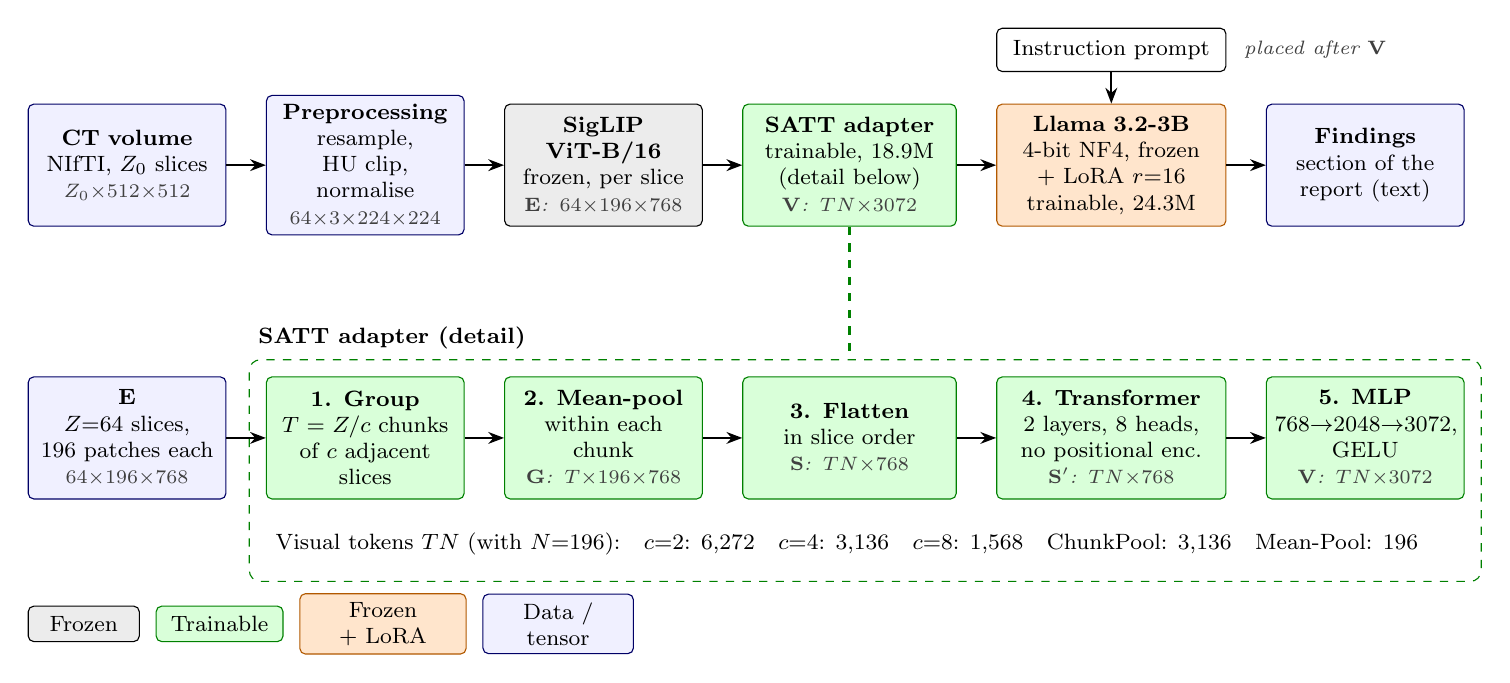
\begin{tikzpicture}[
  font=\footnotesize,
  box/.style={draw, rounded corners=2pt, align=center, minimum height=1.55cm,
              inner sep=3pt, text width=2.3cm},
  frozen/.style={box, fill=gray!15},
  train/.style={box, fill=green!15, draw=green!50!black},
  lora/.style={box, fill=orange!20, draw=orange!70!black},
  data/.style={box, fill=blue!6, draw=blue!40!black},
  arr/.style={-{Stealth[length=2mm]}, thick},
  dimlab/.style={font=\scriptsize\itshape, text=black!75},
  node distance=0.5cm
]
% --- top row: end-to-end pipeline ---
\node[data] (ct) {\textbf{CT volume}\\NIfTI, $Z_0$ slices\\\tsh{$Z_0{\times}512{\times}512$}};
\node[data, right=of ct] (pre) {\textbf{Preprocessing}\\resample, HU clip,\\normalise\\\tsh{$64{\times}3{\times}224{\times}224$}};
\node[frozen, right=of pre] (enc) {\textbf{SigLIP ViT-B/16}\\frozen, per slice\\\tsh{$\mathbf{E}$: $64{\times}196{\times}768$}};
\node[train, right=of enc, text width=2.5cm] (satt) {\textbf{SATT adapter}\\trainable, 18.9M\\(detail below)\\\tsh{$\mathbf{V}$: $TN{\times}3072$}};
\node[lora, right=of satt, text width=2.7cm] (llm) {\textbf{Llama 3.2-3B}\\4-bit NF4, frozen\\+ LoRA $r{=}16$\\trainable, 24.3M};
\node[data, right=of llm] (out) {\textbf{Findings}\\section of the\\report (text)};
\node[box, fill=white, above=0.4cm of llm, text width=2.7cm, minimum height=0.55cm] (prompt) {Instruction prompt};

\draw[arr] (ct) -- (pre);
\draw[arr] (pre) -- (enc);
\draw[arr] (enc) -- (satt);
\draw[arr] (satt) -- (llm);
\draw[arr] (prompt) -- (llm);
\draw[arr] (llm) -- (out);
\node[dimlab, anchor=west] at ($(prompt.east)+(0.1,0)$) {placed after $\mathbf{V}$};

% --- bottom row: SATT detail ---
\node[data, below=1.9cm of ct] (e) {$\mathbf{E}$\\$Z{=}64$ slices,\\196 patches each\\\tsh{$64{\times}196{\times}768$}};
\node[train, right=of e] (grp) {\textbf{1. Group}\\$T=Z/c$ chunks\\of $c$ adjacent\\slices};
\node[train, right=of grp] (pool) {\textbf{2. Mean-pool}\\within each chunk\\\tsh{$\mathbf{G}$: $T{\times}196{\times}768$}};
\node[train, right=of pool, text width=2.5cm] (flat) {\textbf{3. Flatten}\\in slice order\\\tsh{$\mathbf{S}$: $TN{\times}768$}};
\node[train, right=of flat, text width=2.7cm] (tr) {\textbf{4. Transformer}\\2 layers, 8 heads,\\no positional enc.\\\tsh{$\mathbf{S}'$: $TN{\times}768$}};
\node[train, right=of tr] (mlp) {\textbf{5. MLP}\\$768{\to}2048{\to}3072$,\\GELU\\\tsh{$\mathbf{V}$: $TN{\times}3072$}};

\draw[arr] (e) -- (grp);
\draw[arr] (grp) -- (pool);
\draw[arr] (pool) -- (flat);
\draw[arr] (flat) -- (tr);
\draw[arr] (tr) -- (mlp);

\node[font=\footnotesize, anchor=north west] (tok) at ($(grp.south west)+(0,-0.3)$)
  {Visual tokens $TN$ (with $N{=}196$):\quad $c{=}2$: 6,272\quad $c{=}4$: 3,136\quad $c{=}8$: 1,568\quad ChunkPool: 3,136\quad Mean-Pool: 196};

\begin{scope}[on background layer]
\node[draw=green!50!black, dashed, rounded corners, fit=(grp)(mlp)(tok), inner sep=6pt] (detail) {};
\end{scope}
\node[font=\footnotesize\bfseries, anchor=south west] at (detail.north west) {SATT adapter (detail)};
\draw[dashed, green!50!black, thick] (satt.south) -- (satt.south |- detail.north);

% --- legend ---
\node[frozen, text width=1.2cm, minimum height=0.45cm, anchor=north west] (lf) at ($(e.west |- detail.south)+(0,-0.3)$) {Frozen};
\node[train, text width=1.4cm, minimum height=0.45cm, right=0.2cm of lf] (lt) {Trainable};
\node[lora, text width=1.9cm, minimum height=0.45cm, right=0.2cm of lt] (ll) {Frozen + LoRA};
\node[data, text width=1.7cm, minimum height=0.45cm, right=0.2cm of ll] (ld) {Data / tensor};
\end{tikzpicture}}
\caption{SATT pipeline (top) and adapter detail (bottom). Each of the 64
preprocessed slices is encoded independently by a frozen SigLIP encoder. The
adapter groups adjacent slices into chunks of size $c$, averages within each
chunk, models the ordered sequence with a two-layer Transformer and projects
it into the language model's embedding space. The mean-pooling baseline
replaces steps 1--4 with a single average over all 64 slices (196 tokens) and
keeps the same MLP. The ChunkPool control skips step 4 only (3,136 tokens at $c=4$). Tensor shapes omit the batch dimension.}
\label{fig:architecture}
\end{figure*}
% ---------------------------------------------------------------------------

\subsection{SATT Adapter}\label{sec:method}
Figure~\ref{fig:architecture} shows the pipeline. The adapter maps
$\mathbf{E}\in\mathbb{R}^{Z\times N\times D_v}$ to visual tokens
$\mathbf{V}\in\mathbb{R}^{TN\times D_l}$ in four steps.

\textbf{Grouping and pooling.} Adjacent slices are grouped into $T=Z/c$
non-overlapping chunks and averaged:
\begin{equation}
\mathbf{G}_t=\frac{1}{c}\sum_{i=(t-1)c+1}^{tc}\mathbf{E}_i,\qquad
t=1,\dots,T,
\end{equation}
giving $\mathbf{G}\in\mathbb{R}^{T\times N\times D_v}$. Pooling before the
Transformer reduces the sequence length by a factor of $c$, and with it the
quadratic cost of self-attention. The cost is that variation within a chunk
is averaged away: a finding visible on only one of the $c$ slices is
attenuated. Larger $c$ therefore means cheaper attention and coarser
resolution along the body axis.

\textbf{Sequence modelling.} $\mathbf{G}$ is flattened in slice order to
$\mathbf{S}\in\mathbb{R}^{TN\times D_v}$ and passed through a two-layer,
eight-head Transformer encoder~\cite{transformer} (feed-forward dimension
2048, dropout 0.1):
\begin{equation}
\mathbf{S}'=\mathrm{TransformerEncoder}(\mathbf{S}),\qquad
\mathbf{S}'\in\mathbb{R}^{TN\times D_v}.
\end{equation}
\textbf{Positional encoding.} No positional encoding is added inside the
adapter. Each token still carries its position \emph{within} its slice,
because SigLIP adds a learned in-plane position embedding to its patches
before encoding them. Nothing in a token records its position \emph{along}
the body axis, that is, which chunk it came from. Self-attention without
positional encoding is permutation-equivariant: permuting the input tokens
permutes the outputs in the same way and changes nothing else. The adapter's
Transformer can therefore exchange information between chunks, but it cannot
use their order; it cannot, for example, learn that one structure lies above
another. Axial order is not lost, however. The tokens leave the adapter in
slice order, and the language model applies its own rotary position
encoding~\cite{roformer} to the whole input sequence, so the order is
available to the language model and to the LoRA weights trained in Phase~2.
We chose this as the simplest design. Its limitation is that any use of axial
position has to be learned inside the language model rather than in the
adapter. An axial positional encoding added to each chunk would remove this
limitation at negligible cost ($T\times D_v$ parameters, 12,288 for $c=4$),
but we did not test it (Section~\ref{sec:limitations}).

\textbf{Projection.} A two-layer MLP with GELU activation maps each token to
the language model's embedding space:
\begin{equation}
\mathbf{V}=W_2\,\mathrm{GELU}(W_1\mathbf{S}'+b_1)+b_2,\qquad
\mathbf{V}\in\mathbb{R}^{TN\times D_l},
\end{equation}
with $W_1\in\mathbb{R}^{2048\times 768}$ and
$W_2\in\mathbb{R}^{3072\times 2048}$. The adapter has 18.9M parameters,
independent of $c$ (11.0M in the Transformer, 7.9M in the MLP;
Table~\ref{tab:params}).

\textbf{Chunk sizes.} We evaluate $c\in\{2,4,8\}$, powers of two that divide
$Z=64$ and give 6,272, 3,136 and 1,568 visual tokens. We did not test $c=1$
(12,544 tokens): training at $c=2$ already required gradient checkpointing to
fit in memory and took 73\,h for Phase~2. Larger chunks ($c\ge16$) and
overlapping windows were not tested.

\subsection{Baselines}
\textbf{Mean-pooling baseline.} This baseline replaces grouping, pooling and
the Transformer with a single average over all slices,
$\mathbf{V}_{\text{base}}=\mathrm{MLP}\big(\tfrac{1}{Z}\sum_{z=1}^{Z}\mathbf{E}_z\big)\in\mathbb{R}^{N\times D_l}$,
producing 196 tokens. It uses the same vision encoder, MLP, language model,
prompt, training schedule and decoding. On its own, however, it differs from
SATT in two ways at once: it has 16 times fewer visual tokens than SATT with
$c=4$, and it has no Transformer.

\textbf{Chunk-pooling control (ChunkPool).} To separate these two factors we
trained an intermediate configuration that keeps SATT's grouping and pooling
with $c=4$ but removes the Transformer:
$\mathbf{V}_{\text{cp}}=\mathrm{MLP}(\mathbf{S})\in\mathbb{R}^{TN\times D_l}$,
with $\mathbf{S}$ as in Section~\ref{sec:method}. It therefore has exactly the
same 3,136 visual tokens as SATT $c=4$, and the same 7.9M-parameter adapter as
the mean-pooling baseline. Comparing SATT $c=4$ with ChunkPool isolates the
effect of the Transformer at a fixed token count; comparing ChunkPool with the
mean-pooling baseline isolates the effect of keeping 16 chunks instead of one
global average, without a Transformer. ChunkPool was trained with the same
two-phase schedule, settings and data as the other configurations.

\subsection{Language Model and Training}
The language model is Llama~3.2-3B-Instruct~\cite{llama3}. In Phase~2 it is
quantized to 4-bit NF4 and fine-tuned with QLoRA~\cite{qlora}; in Phase~1,
where it is fully frozen, it is kept in bfloat16. The visual tokens are placed before a fixed
instruction prompt, and the model is trained with the next-token
cross-entropy loss on the findings text only. Following the two-stage recipe
of LLaVA~\cite{llava,llava15}, training has two phases.
\textbf{Phase~1 (alignment)}: only the adapter is trained; the vision encoder
and language model are frozen. \textbf{Phase~2 (fine-tuning)}: the adapter
and LoRA weights~\cite{lora} are trained jointly. Aligning the randomly
initialised adapter first avoids passing its early, uninformative gradients
into the LoRA weights. We did not run a single-phase control. Table~\ref{tab:training}
lists all settings. The values are standard choices for QLoRA fine-tuning
and were not tuned. For each configuration we keep the Phase~2 checkpoint
with the lowest validation loss. For the four main configurations this was
the same epoch, with losses between 1.024 and 1.027; for ChunkPool it was the
final (fifth) epoch, with loss 1.024. All configurations were trained on one NVIDIA RTX
6000 Ada GPU (48\,GB).

\begin{table}[t]
\centering
\caption{Training settings, identical for all configurations except where
noted.}
\label{tab:training}
\footnotesize
\resizebox{\columnwidth}{!}{%
\begin{tabular}{@{}lll@{}}
\toprule
\textbf{Setting} & \textbf{Phase 1} & \textbf{Phase 2} \\
\midrule
Trainable parts & adapter & adapter + LoRA \\
Trainable parameters & 18.9M$^{a}$ & 43.2M$^{a}$ \\
Optimiser & AdamW (wd 0.01) & AdamW (wd 0.01) \\
Learning rate & $1\times10^{-4}$ & $2\times10^{-5}$ \\
Batch $\times$ accumulation & $2\times4$ (effective 8)$^{b}$ & $1\times8$ (effective 8) \\
Epochs & 3 & 5 (best by val.\ loss) \\
Gradient clipping & 1.0 & 1.0 \\
Max.\ text length & 512 tokens & 512 tokens \\
LoRA & --- & $r=16$, $\alpha=32$, 7 projections \\
Language model precision & bfloat16 & 4-bit NF4 \\
\bottomrule
\end{tabular}}

\vspace{2pt}
\parbox{\columnwidth}{\scriptsize $^{a}$For SATT; Table~\ref{tab:params}
gives the counts for every component and configuration.
$^{b}$$1\times8$ for $c=2$ in Phase~1. Gradient checkpointing was used in
Phase~2 for $c=2$ and for ChunkPool, which was trained later with a code
version that enables it by default; it changes memory use and speed, not the
computed gradients (up to floating-point rounding).}
\end{table}

\textbf{Parameter counts.} Table~\ref{tab:params} lists every component.
Only the adapter and the LoRA weights are trained. The SATT adapter has
18.9M parameters, 11.0M in the Transformer and 7.9M in the MLP, and this
count does not depend on $c$, because pooling has no parameters and the
Transformer's weights do not depend on sequence length. The mean-pooling
and ChunkPool adapters are the MLP alone (7.9M each). LoRA adds 24.3M parameters to the frozen
3.21B-parameter language model, which is 0.76\% of the language model, or
0.75\% of the language model including LoRA (3.24B), the figure reported by
the PEFT library. In Phase~2 the trainable total is therefore 43.2M for SATT
and 32.2M for the mean-pooling baseline and ChunkPool, 1.29\% and 0.96\% of the whole
system of about 3.35B parameters.

\begin{table}[t]
\centering
\caption{Parameter counts. Frozen components are identical in all
configurations.}
\label{tab:params}
\footnotesize
\setlength{\tabcolsep}{4pt}
\resizebox{\columnwidth}{!}{%
\begin{tabular}{@{}llr@{}}
\toprule
\textbf{Component} & \textbf{Status} & \textbf{Parameters} \\
\midrule
SigLIP ViT-B/16 vision encoder$^{a}$ & frozen & 92.9M \\
Llama 3.2-3B-Instruct (4-bit) & frozen & 3,212.7M \\
\midrule
SATT adapter (any $c$) & trainable & 18.9M \\
\quad Transformer encoder (2 layers) & & 11.0M \\
\quad MLP projector & & 7.9M \\
Mean-pooling or ChunkPool adapter (MLP only) & trainable & 7.9M \\
LoRA ($r=16$, 7 projections, 28 layers) & trainable (Phase 2) & 24.3M \\
\midrule
\multicolumn{2}{@{}l}{Phase 2 trainable, SATT (adapter + LoRA)} & 43.2M \\
\multicolumn{2}{@{}l}{Phase 2 trainable, mean-pooling or ChunkPool} & 32.2M \\
\multicolumn{2}{@{}l}{Whole system, SATT} & 3,348.8M \\
\bottomrule
\end{tabular}}

\vspace{2pt}
\parbox{\columnwidth}{\scriptsize LoRA is 0.76\% of the language model's
3,212.7M parameters (0.75\% of 3,237.1M including LoRA). Phase-2 trainable
parameters are 1.29\% (SATT) and 0.96\% (mean-pooling, ChunkPool) of the whole system.
$^{a}$Includes a 7.1M-parameter pooling head that is loaded but not used; the
patch features come from the 85.8M-parameter encoder before it.}
\end{table}

\subsection{Decoding}
Reports are generated greedily with at most 600 new tokens. Decoding
constraints against repetition, such as the repetition
penalty~\cite{ctrl} and blocking of repeated $n$-grams~\cite{paulus2018}, are
common defaults because greedy decoding tends to loop~\cite{holtzman2020}.
Structured radiology reports, however, legitimately repeat short statements
such as ``Normal.'' across organ sections. We therefore selected the decoding
setting on 100 \emph{validation} scans with the $c=4$ model, comparing four
settings, and chose the one with the highest RadGraph-F1, a criterion fixed
in advance (Section~\ref{sec:decoding}). The chosen setting, a repetition
penalty of 1.1 with no $n$-gram blocking, was then used once for all five
configurations on the test set.

\subsection{Evaluation Protocol}
All configurations are evaluated on the same 1,000 test scans, drawn at
random from the 5,123 available test scans with seed 42, fixed before any
evaluation. Generating a report takes 10--15\,s per scan, so evaluating all
five configurations on the full test split was not feasible on our shared
cluster. To check that the subset is representative, we compared it with the
remaining 4,123 test scans: reference report length did not differ
(Kolmogorov--Smirnov $D=0.022$, $p=0.81$), and the frequency of ten common
findings and terms differed by at most 1.5 percentage points (all
$\chi^2$ $p>0.3$).

\textbf{Metrics.} We report BLEU-4~\cite{bleu} (computed with
sacreBLEU~\cite{sacrebleu}), ROUGE-1, ROUGE-2 and ROUGE-L~\cite{rouge},
METEOR~\cite{meteor}, ClinicalBERT-F1, a BERTScore~\cite{bertscore} computed
with the Bio\_ClinicalBERT encoder~\cite{clinicalbert}, and
RadGraph-F1~\cite{radgraph,f1radgraph}, computed with the RadGraph-XL
model~\cite{radgraphxl} at the entity-and-relation level. All metrics lie in
$[0,1]$, and higher is better. The first five measure word overlap with the
reference. ClinicalBERT-F1 measures semantic similarity, and RadGraph-F1
measures agreement on clinical entities (anatomy and observations, present,
absent or uncertain) and the relations between them, which makes it the most
clinically meaningful of the seven.

\textbf{Statistics.} We compute 95\% confidence intervals with the percentile
bootstrap~\cite{efron1993}, resampling the 1,000 test scans with replacement
(10,000 resamples; 2,000 for corpus-level BLEU-4). Configurations are
compared with the paired bootstrap~\cite{koehn2004}, using the same resampled
scans for both. These intervals capture variation due to the choice of test
scans. They do not capture variation between training runs, because each
configuration was trained once.

% ===========================================================================
\section{Results}

\subsection{Effect of Slice-Aware Tokenization (RQ1)}

Table~\ref{tab:main} reports all metrics with confidence intervals, and
Table~\ref{tab:paired} the paired differences. SATT with $c=4$ improves on
the mean-pooling baseline in RadGraph-F1 by 0.019 (95\% CI [0.015, 0.023]),
from 0.312 to 0.331, a relative gain of about 6\%. It also improves BLEU-4,
ROUGE-1, ROUGE-L, METEOR and ClinicalBERT-F1, but not ROUGE-2, where the
difference is 0.003 with an interval that includes zero. The answer to the
first part of RQ1 is therefore positive but modest: a consistent,
statistically separable improvement on this test set, but not a large one.

The ChunkPool control answers the second part (Table~\ref{tab:paired},
second and third columns). With the same 3,136 visual tokens, removing the
Transformer lowers RadGraph-F1 by 0.023 (CI [0.019, 0.027]), from 0.331 to
0.308, and lowers all seven metrics, each with an interval that excludes
zero. Keeping 16 chunks instead of one global average does not help without
the Transformer: ChunkPool is slightly below the mean-pooling baseline on
RadGraph-F1 ($-0.004$, CI [$-0.007$, $-0.0003$]), better on BLEU-4, ROUGE-1
and METEOR, and worse on ROUGE-2 and ROUGE-L. On this test set, therefore,
SATT's improvement over mean pooling comes from the Transformer applied to
the chunk sequence, not from the larger number of visual tokens alone. One
possible reason is that without the Transformer each token is a projection of
a single pooled patch, and relating thousands of such tokens is left entirely
to the language model; we did not test this explanation. Two qualifications
apply. Each configuration was trained once, so these differences may be
partly within run-to-run variation (Section~\ref{sec:limitations}). And we
tested the Transformer only on chunked input ($c=4$), not on the 196
mean-pooled tokens.

\begin{table*}[t]
\centering
\caption{Test-set results on 1,000 scans (higher is better). Values are point
estimates with 95\% bootstrap confidence intervals. All metrics on a
$[0,1]$ scale. Best value per column in bold.}
\label{tab:main}
\footnotesize
\setlength{\tabcolsep}{4pt}
\resizebox{\textwidth}{!}{%
\begin{tabular}{@{}lccccccc@{}}
\toprule
\textbf{Configuration} & \textbf{BLEU-4} & \textbf{ROUGE-1} & \textbf{ROUGE-2} &
\textbf{ROUGE-L} & \textbf{METEOR} & \textbf{ClinicalBERT-F1} & \textbf{RadGraph-F1} \\
\midrule
Mean-Pool (196 tokens)
 & 0.104 \ci{0.097}{0.111} & 0.380 \ci{0.373}{0.386} & 0.204 \ci{0.197}{0.211}
 & 0.283 \ci{0.276}{0.290} & 0.258 \ci{0.251}{0.266} & 0.809 \ci{0.807}{0.811}
 & 0.312 \ci{0.304}{0.320} \\
ChunkPool $c=4$, no Transformer (3,136)
 & 0.118 \ci{0.111}{0.126} & 0.395 \ci{0.388}{0.401} & 0.194 \ci{0.188}{0.200}
 & 0.277 \ci{0.271}{0.283} & 0.275 \ci{0.268}{0.283} & 0.808 \ci{0.806}{0.810}
 & 0.308 \ci{0.301}{0.316} \\
\midrule
SATT $c=8$ (1,568)
 & 0.097 \ci{0.090}{0.104} & 0.388 \ci{0.380}{0.395} & 0.206 \ci{0.199}{0.213}
 & 0.288 \ci{0.281}{0.295} & 0.267 \ci{0.260}{0.275} & 0.810 \ci{0.808}{0.812}
 & 0.316 \ci{0.308}{0.324} \\
SATT $c=4$ (3,136)
 & \textbf{0.142} \ci{0.135}{0.150} & \textbf{0.411} \ci{0.405}{0.418} & \textbf{0.206} \ci{0.199}{0.214}
 & \textbf{0.291} \ci{0.284}{0.298} & \textbf{0.286} \ci{0.279}{0.293} & 0.813 \ci{0.811}{0.815}
 & \textbf{0.331} \ci{0.323}{0.339} \\
SATT $c=2$ (6,272)
 & 0.119 \ci{0.112}{0.126} & 0.403 \ci{0.396}{0.409} & 0.201 \ci{0.195}{0.208}
 & 0.286 \ci{0.279}{0.292} & 0.265 \ci{0.258}{0.272} & \textbf{0.814} \ci{0.812}{0.816}
 & 0.328 \ci{0.320}{0.336} \\
\bottomrule
\end{tabular}}
\end{table*}

\begin{table*}[t]
\centering
\caption{Paired differences on the same 1,000 test scans (A $-$ B), with 95\%
bootstrap confidence intervals. $^{\ast}$Interval excludes zero. The second
and third columns use the ChunkPool control: same tokens as $c=4$ without the
Transformer.}
\label{tab:paired}
\footnotesize
\setlength{\tabcolsep}{3pt}
\resizebox{\textwidth}{!}{%
\begin{tabular}{@{}lccccc@{}}
\toprule
& \multicolumn{3}{c}{\textbf{SATT versus baselines}} & \multicolumn{2}{c}{\textbf{Chunk size}} \\
\cmidrule(lr){2-4}\cmidrule(l){5-6}
\textbf{Metric} & \textbf{$c{=}4$ $-$ Mean-Pool} & \textbf{$c{=}4$ $-$ ChunkPool} & \textbf{ChunkPool $-$ Mean-Pool} & \textbf{$c{=}4$ $-$ $c{=}8$} & \textbf{$c{=}2$ $-$ $c{=}4$} \\
& \scriptsize(SATT gain) & \scriptsize(effect of Transformer) & \scriptsize(effect of chunking alone) & & \\
\midrule
RadGraph-F1 & $+0.019^{\ast}$ \ci{0.015}{0.023} & $+0.023^{\ast}$ \ci{0.019}{0.027} & $-0.004^{\ast}$ \ci{-0.007}{-0.0003} & $+0.015^{\ast}$ \ci{0.011}{0.019} & $-0.004$ \ci{-0.008}{0.0002} \\
BLEU-4 & $+0.038^{\ast}$ \ci{0.034}{0.043} & $+0.024^{\ast}$ \ci{0.019}{0.028} & $+0.015^{\ast}$ \ci{0.010}{0.019} & $+0.045^{\ast}$ \ci{0.041}{0.049} & $-0.023^{\ast}$ \ci{-0.027}{-0.019} \\
ROUGE-1 & $+0.032^{\ast}$ \ci{0.027}{0.036} & $+0.017^{\ast}$ \ci{0.012}{0.021} & $+0.015^{\ast}$ \ci{0.010}{0.020} & $+0.024^{\ast}$ \ci{0.019}{0.029} & $-0.009^{\ast}$ \ci{-0.013}{-0.004} \\
ROUGE-2 & $+0.003$ \ci{-0.001}{0.006} & $+0.013^{\ast}$ \ci{0.009}{0.017} & $-0.010^{\ast}$ \ci{-0.013}{-0.007} & $+0.001$ \ci{-0.003}{0.004} & $-0.005^{\ast}$ \ci{-0.009}{-0.002} \\
ROUGE-L & $+0.008^{\ast}$ \ci{0.005}{0.012} & $+0.014^{\ast}$ \ci{0.010}{0.017} & $-0.006^{\ast}$ \ci{-0.009}{-0.002} & $+0.003$ \ci{-0.0004}{0.007} & $-0.005^{\ast}$ \ci{-0.009}{-0.002} \\
METEOR & $+0.027^{\ast}$ \ci{0.023}{0.032} & $+0.010^{\ast}$ \ci{0.006}{0.015} & $+0.017^{\ast}$ \ci{0.013}{0.021} & $+0.018^{\ast}$ \ci{0.014}{0.022} & $-0.021^{\ast}$ \ci{-0.025}{-0.017} \\
ClinicalBERT-F1 & $+0.004^{\ast}$ \ci{0.003}{0.005} & $+0.005^{\ast}$ \ci{0.004}{0.007} & $-0.001$ \ci{-0.002}{0.000} & $+0.003^{\ast}$ \ci{0.002}{0.004} & $+0.001$ \ci{-0.001}{0.002} \\
\bottomrule
\end{tabular}}
\end{table*}

\subsection{Effect of Chunk Size and Computational Cost (RQ2)}

Report quality is not monotonic in chunk size (Table~\ref{tab:main}). $c=4$
is best on six of seven metrics. $c=8$ is close to the mean-pooling baseline,
and $c=2$ is either worse than $c=4$ or not distinguishable from it. On
RadGraph-F1, $c=2$ and $c=4$ cannot be separated (difference $-0.004$, CI
$[-0.008, 0.000]$). Halving the chunk from 8 to 4 helps, but halving it again
does not. A plausible explanation is that, beyond a point, a longer visual
sequence makes the adapter's attention harder to train with the same data
and schedule. We do not test this explanation here, and because each model
was trained once, the ordering of $c=2$ and $c=4$ in particular may not hold
across training runs.

Table~\ref{tab:cost} reports the cost of each configuration. Phase-2
training time grows faster than the token count: from 12.3\,h at $c=8$ to
26.5\,h at $c=4$ (2.0$\times$ the tokens, 2.2$\times$ the time) and 73.4\,h
at $c=2$, where gradient checkpointing also adds recomputation. Self-attention
over $L=TN$ tokens costs $O(L^2 D_v)$ per layer; $L$ is 1,568, 3,136 and
6,272 for $c=8$, 4 and 2. Inference is cheap for all configurations: peak GPU
memory is 2.7--4.2\,GB and generation takes 10.5--14.3\,s per scan. Inference
time depends mostly on the length of the generated report rather than on the
number of visual tokens; $c=4$ writes the longest reports and is the slowest.
For RQ2, $c=4$ is the best trade-off in this study: it gives the best quality
at about one third of the Phase-2 training time of $c=2$.

\begin{table}[t]
\centering
\caption{Computational cost per configuration on one NVIDIA RTX 6000 Ada.}
\label{tab:cost}
\footnotesize
\setlength{\tabcolsep}{3pt}
\begin{tabular}{@{}lcccccc@{}}
\toprule
& \textbf{Visual} & \textbf{Trainable} & \textbf{Phase 2} & \textbf{Train} & \textbf{Infer.} & \textbf{Peak} \\
\textbf{Config.} & \textbf{tokens} & \textbf{params} & \textbf{time} & \textbf{samples/s} & \textbf{scans/min} & \textbf{mem.} \\
\midrule
Mean-Pool & 196 & 32.2M & 5.5\,h & 3.9 & 5.3 & 2.7\,GB \\
ChunkPool & 3,136 & 32.2M & 28.8\,h$^{\dagger}$ & 0.7 & 4.8 & 3.4\,GB \\
$c=8$ & 1,568 & 43.2M & 12.3\,h & 1.7 & 5.7 & 3.0\,GB \\
$c=4$ & 3,136 & 43.2M & 26.5\,h & 0.8 & 4.2 & 3.4\,GB \\
$c=2$ & 6,272 & 43.2M & 73.4\,h$^{\dagger}$ & 0.3 & 4.7 & 4.2\,GB \\
\bottomrule
\end{tabular}

\vspace{2pt}
\parbox{\columnwidth}{\scriptsize Trainable parameters are for Phase~2
(adapter + LoRA; Table~\ref{tab:params}); the whole system has about 3.35B parameters in all
configurations. Phase-2 time is wall-clock for 5 epochs including validation;
training samples/s is derived from it. Inference throughput and peak GPU
memory were measured during test-set generation. Phase-1 times are omitted
because several Phase-1 jobs were interrupted and resumed on the shared
cluster. $^{\dagger}$With gradient checkpointing, which trades speed for
memory, so these times are not directly comparable with the others; ChunkPool,
for example, is slower than SATT $c=4$ despite having no Transformer.}
\end{table}

\subsection{Effect of Decoding (RQ3)}\label{sec:decoding}

Two different evaluations appear in this subsection, and
Table~\ref{tab:decoding} keeps them apart. Part~(a) is the selection step: four
decoding settings for the $c=4$ model on 100 \emph{validation} scans. Part~(b)
is the confirmation: the original and the selected setting for the same model
on the 1,000 \emph{test} scans used everywhere else in this paper. The
original setting, used in our initial experiments, is a repetition penalty of
1.3 combined with blocking of repeated 4-grams.

\textbf{Validation (selection).} With the original setting, the model almost
never wrote a plain ``Normal.'' after the first organ section (8\% of later
sections, against 62\% in the references). It instead filled sections with
stereotyped alternatives: 89\% of the 100 reports described the gallbladder as
surgically absent, against 22\% of references, and 98\% contained wording
that refers to earlier examinations (for example ``previously'', ``interval''
or ``unchanged''), although the model never sees one. Removing all
constraints made 21\% of reports loop. A mild penalty of 1.1 without $n$-gram
blocking gave the highest validation RadGraph-F1, 0.338 against 0.237 for the
original setting (paired difference $+0.10$, 95\% CI [0.078, 0.126]), with
2\% looping, and it halved generation time.

\textbf{Test (confirmation).} The selected setting was then applied once to
the test set. For the same $c=4$ model on the same 1,000 test scans,
RadGraph-F1 is 0.244 with the original setting and 0.331 with the selected
one; ROUGE-2 rises from 0.100 to 0.206 and BLEU-4 from 0.112 to 0.142. The
validation and test values differ slightly because they come from different
scans; both show the same effect. All other test-set results in this paper
use the selected setting. For templated report generation, therefore, the
strength of the repetition constraints matters as much as the architectural
choices we compare in Table~\ref{tab:main}.

\begin{table}[t]
\centering
\caption{Effect of decoding settings on SATT $c=4$. (a) Selection on 100
validation scans. (b) Confirmation on the 1,000 test scans. RP: repetition
penalty; NR: size of blocked repeated $n$-grams (0 = none).}
\label{tab:decoding}
\footnotesize
\setlength{\tabcolsep}{3pt}
\begin{tabular}{@{}cccccccc@{}}
\toprule
\multicolumn{8}{@{}l}{\textit{(a) Validation, 100 scans (used to choose the setting)}} \\
\textbf{RP} & \textbf{NR} & \textbf{RadGraph} & \textbf{ROUGE-2} & \textbf{BLEU-4} & \textbf{Loops} & \textbf{``Normal''} & \textbf{s/scan} \\
\midrule
1.3$^{\ast}$ & 4  & 0.237 & 0.098 & 0.107 & 0\%  & 8\%  & 27.6 \\
1.0 & 0  & 0.283 & 0.178 & 0.126 & 21\% & 95\% & 14.3 \\
\textbf{1.1} & \textbf{0}  & \textbf{0.338} & \textbf{0.211} & \textbf{0.153} & 2\%  & 86\% & 14.3 \\
1.0 & 12 & 0.322 & 0.195 & 0.143 & 3\%  & 87\% & 14.1 \\
\midrule
\multicolumn{8}{@{}l}{\textit{(b) Test, 1,000 scans (selected setting applied once)}} \\
1.3$^{\ast}$ & 4 & 0.244 & 0.100 & 0.112 & & & \\
\textbf{1.1} & \textbf{0} & \textbf{0.331} & \textbf{0.206} & \textbf{0.142} & & & 14.3 \\
\bottomrule
\end{tabular}

\vspace{2pt}
\parbox{\columnwidth}{\scriptsize $^{\ast}$Original setting, used in our
initial experiments. Bold: selected setting, used for every other test-set
result in this paper; the bold test row equals the $c=4$ row of
Table~\ref{tab:main}. Loops: reports that repeat one sentence three or more
times. ``Normal'': share of liver, gallbladder, spleen, pancreas and adrenal
sections that consist only of ``Normal.'' (validation references: 62\%).
Loops and ``Normal'' were measured only in the validation pilot.}
\end{table}

\subsection{Context: Published Results on the Same Dataset}

Table~\ref{tab:merlin} lists the published results on the Merlin dataset
alongside ours. The comparison is \emph{not controlled}, for four reasons.
Merlin generated reports one organ section at a time with organ-specific
prompts. It was evaluated on its full 5,137-scan test split, whereas we use a
1,000-scan subset. The Merlin paper does not state the $n$-gram order of its
BLEU score, the implementation of its metrics, or the RadGraph reward level.
Finally, its BERTScore uses a general-domain encoder, unlike our
ClinicalBERT-F1, so we omit that column. The table should be read as context,
not as evidence that one model is better. SATT's word-overlap scores are in a
similar range to Merlin's, its ROUGE-2 is lower and its RadGraph-F1 is
nominally higher. Establishing whether SATT is better or worse than Merlin
would require evaluating both under one protocol.

\begin{table}[t]
\centering
\caption{Published results on the Merlin abdominal CT test data. Not a
controlled comparison; see text.}
\label{tab:merlin}
\footnotesize
\setlength{\tabcolsep}{4pt}
\begin{tabular}{@{}lccc@{}}
\toprule
\textbf{Model} & \textbf{BLEU} & \textbf{ROUGE-2} & \textbf{RadGraph-F1} \\
\midrule
RadFM~\cite{radfm}, as reported in~\cite{merlin} & 0.000 & 0.011 & 0.008 \\
Merlin~\cite{merlin}, as reported & 0.102 & 0.262 & 0.293 \\
SATT $c=4$, this work & 0.142$^{a}$ & 0.206 & 0.331$^{b}$ \\
\bottomrule
\end{tabular}

\vspace{2pt}
\parbox{\columnwidth}{\scriptsize Merlin and RadFM values are for full
reports on 5,137 test scans, as reported in~\cite{merlin}; ours are for 1,000
test scans. $^{a}$BLEU-4; the $n$-gram order is not stated in~\cite{merlin}.
$^{b}$Entity-and-relation level; the level used in~\cite{merlin} is not
stated.}
\end{table}

\subsection{Error Analysis (RQ3)}

We distinguish four related kinds of error. A \emph{factual error}
contradicts the reference, for example calling a present gallbladder absent.
\emph{Unsupported information} cannot be derived from the model's input
whether or not it happens to be true, for example a comparison with a prior
examination or a citation of an original image number. An \emph{omission}
leaves out a finding that the reference reports. A \emph{potentially
clinically significant} error is any of these that could change management,
such as missing a mass. ``Hallucination'' covers the first two. We report
counts of each kind that can be measured automatically. Judging clinical
significance requires a radiologist, which this study did not include.

Table~\ref{tab:errors} gives the counts on the 1,000 test scans. RadGraph
entity counts show that \textbf{omission is the dominant error}. Every
configuration mentions about 12--16 positive findings per report against 39
in the references, and only 11--13\% of the reference's positive findings
appear in the generated report, matched by exact entity text. This measure
undercounts paraphrases, so the true recall is somewhat higher, but the
three-fold gap in the number of findings does not depend on matching.
Generated reports are also less than half as long as the references (114--160
words against 303). Merlin's authors report the same tendency to under-report
positive findings~\cite{merlin}.

\begin{table}[t]
\centering
\caption{Error analysis on 1,000 test scans. Findings are RadGraph
observation entities; precision and recall use exact-text matching and are
approximate.}
\label{tab:errors}
\footnotesize
\setlength{\tabcolsep}{2.5pt}
\resizebox{\columnwidth}{!}{%
\begin{tabular}{@{}lcccccc@{}}
\toprule
& \textbf{Ref.} & \textbf{Mean-Pool} & \textbf{ChunkPool} & \textbf{$c{=}8$} & \textbf{$c{=}4$} & \textbf{$c{=}2$} \\
\midrule
Words per report & 303 & 121 & 136 & 114 & 160 & 136 \\
Positive findings / report & 39.1 & 12.9 & 15.8 & 11.6 & 12.6 & 13.2 \\
Negated findings / report & 10.1 & 4.6 & 4.9 & 4.4 & 7.2 & 6.8 \\
Positive-finding precision & --- & 0.33 & 0.31 & 0.38 & 0.36 & 0.36 \\
Positive-finding recall & --- & 0.11 & 0.13 & 0.11 & 0.12 & 0.12 \\
\midrule
Gallbladder ``absent'' & 23\% & 29\% & 42\% & 47\% & 10\% & 21\% \\
\quad precision of that claim & --- & 0.35 & 0.36 & 0.33 & 0.35 & 0.37 \\
Prior-study wording$^{b}$ & 66\% & 16\% & 15\% & 9\% & 27\% & 15\% \\
Original image-number citation & 45\% & 26\% & 17\% & 14\% & 33\% & 25\% \\
\bottomrule
\end{tabular}}

\vspace{2pt}
\parbox{\columnwidth}{\scriptsize Gallbladder: share of reports, among those
with a gallbladder section in both texts, stating it is absent. Last two
rows: share of reports containing such wording. Comparisons with earlier
studies and original image numbers cannot be derived from the model's input,
one scan resampled to 64 slices. $^{b}$Words such as ``prior'', ``previously'',
``interval'', ``unchanged'' and ``stable''; the count also includes ``prior''
used for surgical history (e.g.\ ``prior colectomy''), which can be visible
on the scan, so it is an upper bound on unsupported comparisons.}
\end{table}

Unsupported information has become less frequent but has not disappeared.
With the selected decoding, 9--27\% of test reports contain prior-study
wording (Table~\ref{tab:errors}). For comparison, 98\% of the $c=4$ reports
contained such wording with the original decoding, but that figure comes from
the 100-scan validation pilot (Section~\ref{sec:decoding}), not from the test
set, so the two numbers indicate the direction of the change rather than its
exact size. These statements are learned from the radiologists' reports: two
thirds of the test references compare with an earlier study, and the training
reports come from the same population. Factual errors persist as well: when
$c=4$ calls the gallbladder absent, it is right only 35\% of the time.
Table~\ref{tab:cases} shows representative cases.

All counts in this subsection are automatic. RadGraph entity extraction and
the word lists behind Table~\ref{tab:errors} make their own errors, and
neither the error categories nor the clinical-impact column of
Table~\ref{tab:cases} has been checked by a radiologist. They describe what
kinds of error occur and roughly how often; they do not establish how often
an error would matter for a patient.

\begin{table*}[t]
\centering
\caption{Representative errors from SATT $c=4$ on test scans. Clinical impact
is our assessment of potential significance, not a radiologist's judgment.}
\label{tab:cases}
\footnotesize
\begin{tabularx}{\textwidth}{@{}>{\raggedright\arraybackslash}p{1.5cm} Y Y >{\raggedright\arraybackslash}p{2.0cm} >{\raggedright\arraybackslash}p{3.4cm}@{}}
\toprule
\textbf{Case} & \textbf{Reference findings (excerpt)} & \textbf{Generated findings (excerpt)} &
\textbf{Error type} & \textbf{Potential clinical impact} \\
\midrule
1 (gallbladder) & Normal. & Surgically absent. & Factual error & Low: misstates surgical history \\
2 (liver) & Stable multiple hepatic hemangiomas. Suggestion of mild steatosis\ldots{} No intrahepatic biliary ductal dilatation. & Normal. & Omission & Moderate: known lesions not reported \\
3 (liver) & Focal fat near the falciform ligament. Scattered subcentimeter hypodensities too small to characterize but likely cysts. & Normal. & Omission & Low: likely incidental findings \\
4 (bowel) & Status post ileocolectomy\ldots{} bowel wall thickening, submucosal edema and mucosal hyperemia involving the neo-terminal ileum\ldots & Postsurgical changes consistent with prior partial colectomy. Mild wall thickening of the rectum, which may be related to underdistention. & Factual error and omission & Potentially significant: inflammation at the anastomosis missed; wrong site \\
\bottomrule
\end{tabularx}
\end{table*}

% ===========================================================================
\section{Discussion}

\textbf{What improved and what did not.} Slice-aware tokenization at $c=4$
improves over global mean pooling on six of seven metrics, including
RadGraph-F1, and the paired intervals exclude zero. The improvement is
modest, and finer chunking does not add to it. The ChunkPool control shows
where it comes from: with chunking but no Transformer, the 3,136 tokens give
no RadGraph-F1 gain over 196 mean-pooled ones, and ChunkPool writes more positive findings
than any other configuration (15.8 per report) at the lowest precision
(0.31), and calls the gallbladder absent in 42\% of reports
(Table~\ref{tab:errors}). More visual tokens alone did not make the reports
more accurate; the Transformer over the chunk sequence did, by a modest
margin. The largest single gain in
this study came instead from changing the decoding settings, which raised the
test-set RadGraph-F1 of the same $c=4$ model by 0.087 (from 0.244 to 0.331,
Table~\ref{tab:decoding}b).

\textbf{Surface overlap versus clinical content.} BLEU-4 and ROUGE reward
reproducing the reference's wording, which in templated reports is largely
the template itself: organ headings and stock normal statements. A model can
therefore raise these scores by following the template more faithfully,
without describing the scan better. The BLEU-4 gain of $c=4$ indicates that
its reports follow the radiologists' structure and phrasing more closely,
which may matter for readability, but it says little about clinical
correctness. Clinical content
is better reflected by RadGraph-F1 and, most directly, by the finding counts
in Table~\ref{tab:errors}, which show all configurations missing most
findings. Part of $c=4$'s BLEU-4 and METEOR advantage may also come from
writing longer reports than the other configurations.

\textbf{Relation to Merlin.} We do not claim that SATT is better than
Merlin. The published numbers come from a different protocol
(Table~\ref{tab:merlin}), Merlin uses a 7B language model and a CT-pretrained
3D encoder, and its 160 hours of training~\cite{merlin} cover foundation-model
pretraining, which is a different task from our adapter and LoRA training and
not comparable with it.

% ===========================================================================
\section{Limitations}\label{sec:limitations}

\begin{itemize}
\item \textbf{Single dataset and institution.} All data come from one
hospital. We performed no external validation, and results may not hold for
other institutions, scanners or reporting styles.
\item \textbf{Test subset.} We evaluated on 1,000 of 5,123 test scans. The
subset matches the rest of the test split on the characteristics we checked,
but results on the full split may differ slightly.
\item \textbf{Single training run.} Each configuration was trained once, with
one random seed. All confidence intervals and paired tests in this paper
resample the 1,000 test scans, so they measure how much a result depends on
which test cases were chosen. They do not measure how much it would change if
the same configuration were trained again, which can be of similar size for
models of this kind. Differences between chunk sizes of 0.004--0.015
RadGraph-F1, and the 0.019 gain over the baseline, may therefore be partly
within run-to-run variation; establishing them firmly requires several
training runs per configuration.
\item \textbf{Scope of the baseline comparisons.} The ChunkPool control
separates the Transformer from the token count at $c=4$ only, with one
training run. We did not test a Transformer over the 196 mean-pooled tokens,
or ChunkPool at other chunk sizes. ChunkPool was also trained later than the
other configurations, with gradient checkpointing enabled; this changes speed,
not the training procedure.
\item \textbf{No radiologist evaluation.} All results are automatic metrics,
and the error analysis (Tables~\ref{tab:errors} and~\ref{tab:cases}) has not
been validated by radiologists; the clinical-impact judgments are the
authors' own. Automatic metrics do not establish whether a generated report
is clinically correct or useful. Given the under-reporting and factual errors
we observe, the system is not suitable for clinical use, including as an
unsupervised draft.
\item \textbf{No axial positional encoding.} The adapter's Transformer cannot
use the order of the chunks along the body axis (Section~\ref{sec:method}); only
the language model receives that order. We did not test an axial positional
encoding.
\item \textbf{Vision encoder.} SigLIP is pretrained on natural images, not
medical images, which may limit how well the visual tokens represent subtle
findings. A medical-domain encoder could improve grounding.
\item \textbf{Preprocessing.} The 64-slice depth, the $224\times224$
resolution and the soft-tissue HU window were fixed in advance, not tuned.
They discard information about small lesions, the lung bases and bone.
\item \textbf{Prior bias of the language model and the reports.} Statements
that compare with prior studies, and stock phrases, are learned from the
training reports. The generated text reflects these reporting habits as well
as the image.
\item \textbf{Single-scan input.} The model never sees prior examinations,
so it cannot legitimately describe interval change.
\end{itemize}

% ===========================================================================
\section{Conclusion and Future Work}

We proposed SATT, an adapter that tokenizes a 3D abdominal CT volume as an
ordered sequence of pooled slice chunks for a QLoRA-adapted language model,
trainable on a single GPU. In a controlled comparison on 1,000 Merlin test
scans, SATT with a chunk size of four improved RadGraph-F1 over an otherwise
identical mean-pooling adapter by 0.019 (95\% CI [0.015, 0.023]) and improved
five other metrics, but not ROUGE-2. A chunk-pooling control showed that this
gain comes from the Transformer over the chunk sequence: with the same 3,136
tokens and no Transformer, RadGraph-F1 was 0.023 lower and no higher than
with mean pooling. Finer chunking did not help further.
Each configuration was trained once, so these differences are established
across test scans, not across training runs. Relaxing the repetition
constraints (from a penalty of 1.3 with 4-gram blocking to a penalty of 1.1
without blocking) improved the automatic metrics more than any architectural
change we tested, raising test-set RadGraph-F1 from 0.244 to 0.331. Whether
the reports are clinically adequate remains open: by automatic counts they
omit most of the positive findings that radiologists report and still contain
some unsupported statements, and no radiologist has assessed them. Merlin
remains the stronger reference point on ROUGE-2, and no controlled comparison
with it has been made.

In order of priority, future work should: (1) improve factual and clinical
grounding, for example with training objectives that reward correct findings;
(2) introduce evaluation by radiologists, together with clinically grounded
metrics such as GREEN~\cite{green} and RaTEScore~\cite{ratescore};
(3) evaluate on the complete test split with several training runs per
configuration, and extend the ChunkPool control to other chunk sizes and to a
Transformer over mean-pooled tokens; (4) replace the
natural-image encoder with a medical-domain one and add positional encoding
along the body axis; (5) incorporate prior examinations and reports, so that
interval change can be described from evidence; and (6) validate across
institutions and scanner types.

% ===========================================================================
\bibliographystyle{IEEEtran}
\bibliography{refs}

\end{document}
